\chapter{The new FASER Pre-Shower detector (14 pages)}

%The motivation for the need of a completely new Pre-Shower detector in the FASER experiment at CERN has been demonstrated in \note{section ref}. The new detectors aims at both extending the initial Physics program of the experiment by enhancing its sensitivity two photonic finals states such as the di-photo decay product on an ALP, but also reinforce the current measurement and provide additional discrimination power for background rejection. 
%In the following chapter, the aim is to provide to the reader a detailed overview of the designed Pre-Shower detector. The discussion will start from the smallest element of the entire detector complex, the ASIC. A description of the requirements to on its performance followed by a description of its architecture, demonstrating the fulfilment of the requirements will be presented. 
% 
% Scaling up in detector subcomponents a description of the Pre-Shower modules, a sub-component assembling 6 ASICs together on a single entity will be given followed by a description of the Pre-Shower planes, a sub-component assembling 12 Pre-shower Modules together. The layout of the complete detector with the Pre-Shower planes and the slabs or absorber will be presented. 
% 
% Finally the readout and the control of the detector will be discussed, starting with the structure of the readout, explaining how the data is then read-out from the ASIC and processed by the different elements in the readout chain for which a description will also be given. The powering, cooling and interlock systems for the detector will also be presented, concluding the description of the newly installed detector in the FASER experiment. 
% 

The motivation for the development of a completely new Pre-Shower detector for the FASER experiment at CERN has been outlined in \note{section ref}. This upgrade is driven by the need to enhance sensitivity to photonic final states, in particular to enable the detection of long lived particles such as ALPs decaying into two photons. In addition to extending the reach of the FASER physics program, the new detector design could improve the discrimination power against background events and reinforcing the robustness and reach of existing measurements. \\

This chapter presents a detailed description of the new Pre-Shower detector, from its smallest components to its integration into the full FASER detector. The discussion begins with a description of the ASIC whose design is based on the knowledge acquired over the years at the University of Geneva by prototyping monolithic silicon pixel detectors for diverse applications. The ASIC is the smallest yet most essential piece of the detector as it digitises the position, time of passage and deposited charge of the traversing particle into a binary stream of data. The performance requirements for the ASIC are first presented, followed by a technical description of its architecture and the design choices made to satisfy the demanding constraints of the experiment. The data processing inside the ASIC is presented to highlight how the aforementioned parameters are extracted and digitised.  

The description then progresses to higher levels of integration. The Pre-Shower modules, each composed of six ASICs mounted on a single support structure, are introduced. These modules represent the basic building blocks of the system. A full detector plane is then formed by assembling twelve such modules, creating a scalable and modular structure. The mechanical layout of the full detector, including the positioning of the Pre-Shower planes and the absorber slabs used to initiate electromagnetic showers, is discussed and justified by the results of Monte Carlo simulations performed in \note{Cite Chiara's thesis} .

In the final part of the chapter, the focus shifts to the readout and control infrastructure. The architecture of the data acquisition chain is described, starting from the formatting of the digitised data and continuing through the transmission and processing of the data by the Logic Board (LB) and the Active Patch Panel (APP). The Pre-shower Interlock and Monitoring (PIM) module is introduced and its functions described.

Overall, this chapter aims to provide a comprehensive understanding of the design, functionality, and integration of the new Pre-Shower detector, a necessary upgrade of the initial FASER detector layout to enhance and reinforce its discovery potential.
	\clearpage 
	\section{Production ASIC Description  \textcolor{blue}{ 6 pages}}
	The development of the FASER Pre-Shower ASIC started in 2020 when a first 1.7$\times$2.6 mm$^2$ prototype with a matrix of 64 elongated hexagonal pixels with a footprint of 200$\times$50 $\mu$m$^2$, subdivided into five smaller matrices with different levels of integration of the frontend electronics as explained in \cite{FASER_proto0}. This ASIC was designed and produced in order to support the Pre-Shower upgrade proposal . In early 2021 the ASIC was tested and showed very satisfactory results in terms of gain and ENC. This studies confirmed the feasibility of integration of front-end elements inside the sensitive area, still complying with requirements imposed. The results were published in the Journal of Instrumentation in late 2021 and can be found in \cite{FASER_proto0}. \\
	
	A second iteration prior to design and production of the final ASIC leading to a prototype of 15$\times$5.75 mm$^2$ with a matrix of 48$\times$128 (1536 total) pixels of regular hexagonal shape wit a \SI{65}{\micro\meter} side resulting in a pixel pitch of roughly \SI{100}{\micro\meter}. The pixel matrix is subdivided in three 16$\times$128 pixels Super-Columns (SCs) each subdivided into 8$\times$8 pixels Super-Pixels (SPs), each composed of 64 pixels. This architecture choice will later be discuss in section \note{section ref}. The purpose of this \textit{pre-production} prototype was to confirm the functionality of the front-end and digital electronics circuitry for the final ASIC, as well as studying the reliability of the power distribution over a large area ASIC and extract the production yield to infer what it would be for the larger \textit{production} ASIC. 
	
	The studies of this prototype have been published in \note{cite pre-prod paper} and helped refining the design of many components of the front-end circuitry 	exhibiting large mismatches between pixel responses and current leakage degrading the measurement of deposited. Additionally, the functionality of the ASIC readout was verified and the production yield was estimated to be below 70\% and that every ASIC exhibit a below 1\% proportion of problematic pixels, more than acceptable from the imposed requirements. More details on the characteristics and testing of the \textit{pre-production} ASIC will be given in \note{section ref (if done)}. \\
	
	Finally, the design of the \textit{production} ASIC was completed in May 2023 and and delivered in the laboratories on the University of Geneva after the wafers were thinned, back-processed and diced in collaboration with Micro-Packs, in July 2024. In the following section, a description of the requirements of the ASIC performances accompanied by a detailed description of the production ASIC. 
	
		\subsection{Requirements and Specifications \textcolor{red}{ 2 pages}}
		The design requirements on the FASER Pre-Shower \textit{production} ASIC are driven by the Monte Carlo studies performed on the production of ALPs and the topology of di-photon signals combined with simulations of the entire Pre-Shower detector in different layout configurations. The different requirements can often push the design choices in different direction and an overall robustness and design simplicity often dictates the direction of development. Some other specifications of the ASIC meet requirements also because of the previously acquired knowledge and widely tested structures in other projects by the design group of the University of Geneva. 
		
		\subsubsection{ASIC footprint}
		The \SI{20}{\centi\meter} aperture of the magnets of the FASER detector defines the total area the new Pre-Shower detector needs to cover. While from the Physics point of view, an ASIC as large as possible would represent the ideal case in terms of non-active area, from the electronics point of view a smaller ASIC represent a larger yield as the probability of failure scales from one ASIC to the other to the power of the ratio in areas. Since ASICs are typically fabricated in rectangular shapes, the circular aperture must be instrumented using an array of identical rectangular sub-elements. As a result, some regions within the aperture may remain uninstrumented due to geometric constraints, while certain areas outside the nominal acceptance may inadvertently be covered. The size of the ASIC is then both driven by an optimised paving of the area available of a silicon wafer and by the need to provide modularity of the sub-elements of the Pre-Shower while keeping a total area leading to sufficient production yield. 
		
		\begin{figure}[h]
			\centering
			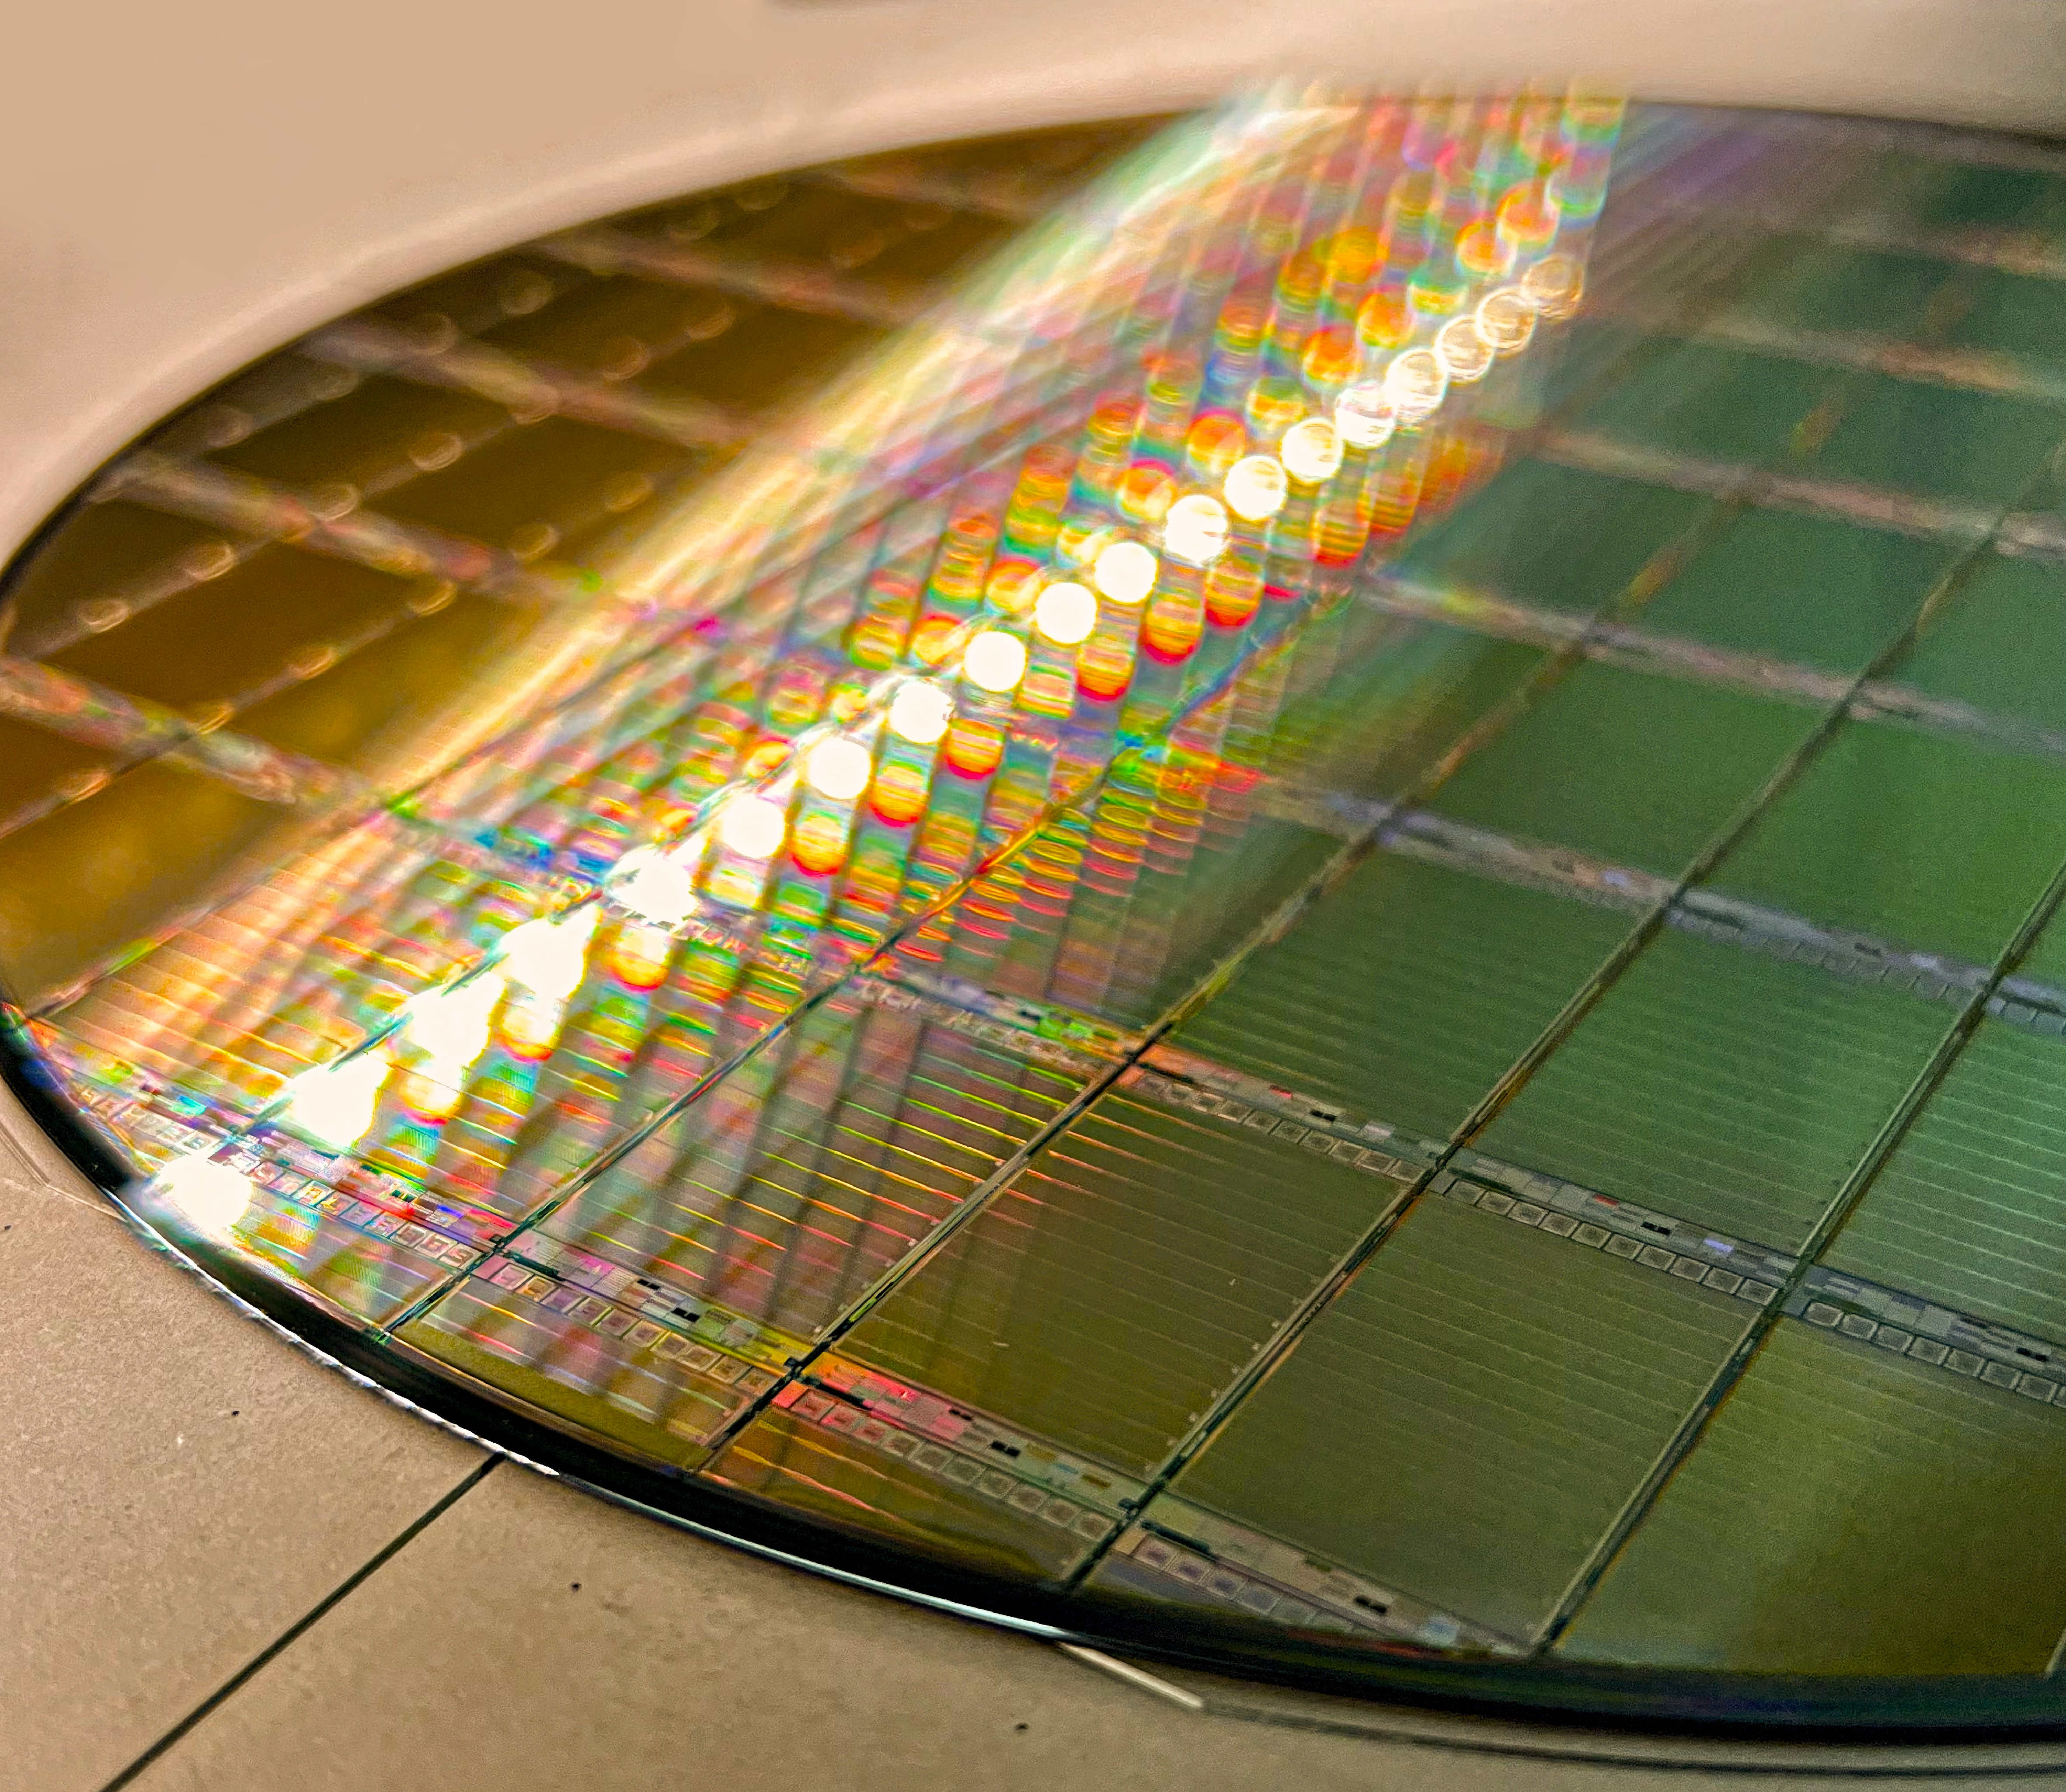
\includegraphics[width=0.9\textwidth]{files/FASER_prod_wafer}
			\caption{Microscope stitched image of the FASER \textit{production} ASIC. The sub-structures of the ASIC can be identified such as the digital peripheries or contact metallic pads (rectangular grey pad on the top and bottom edge). The 13 vertical lines are the digital columns.}
			\label{im:FASER_prod_wafer}
		\end{figure}
		
		The \textit{production} ASIC has a total footprint of 22.15$\times$15.35 mm$^2$ with an active area covering 21.61$\times$14.36 mm$^2$ for a total of roughly 91\% of the ASIC area being active, hence resulting in 9\% of so-called "dead-area" mostly composed of the ASIC periphery. In addition, the dead area is also composed by 13 thin column going across the ASIC small side, also called the digital column. This structure has a pitch of roughly half the pixels pitch (\SI{60}{\micro\meter}) and contributes at the level of 3\% to the dead-area. A thoughtful assembly of ASICs together to pave the aperture of the magnet has to be made, it will be discussed in \note{ref to section on plane.} 
		The choice in size of the pixels composing the 208$\times$128 matrix was mainly driven by the already existing pixel design with hexagonal pixels wit a side of \SI{65}{\micro\meter} for a pitch on both direction of roughly \SI{100}{\micro\meter}. The ALP Monte Carlo simulation exhibited a clear dependence on the rate of di-photon signals as a function of the required separation between showers initiated by the two photons, hence reducing the sensitivity reach. At first order, one can distinguish two different shower cores if there is at least one pixel separating the pixel containing the core of the showers, this leads to a separation between the photons of at least \SI{200}{\micro\meter}, for which the sensitivity reach is given as the second outermost line in figure \ref{im:reach_plot_detector}. The many different design challenges associated to a reduced pixel pitch did not justify a sufficient improvment of the performances in terms of sensitivity reach. 
		
		\subsubsection{High dynamic range}
		The performance of the new Pre-Shower lies in its ability to distinguish the cores of the electromagnetic showers produced by two close-by photons. As the photons have significant boost due to their very high energy, the core of the shower will remain narrow while the shower spread, depending mostly on secondaries with higher transverse momentum, will remain the same as it only depends on the amount of radiation length crossed and the critical energy in the medium in which the showers develops \cite{PDG}. In order to quantify the range of deposited charge in a single pixel, Monte Carlo simulations of incident photons with energies sampled from the ALP production simulations were realised. The studies are presented in \cite{Kotitsa_thesis} and an interesting result is adapted in figure \ref{im:charge_per_plane_FASER}. The figure displays the distribution of the maximum charge recorded in a pixel (corresponding roughly to the charge of the core of the shower) for each plane in the FASER Pre-Shower.
		
		\begin{figure}[h]
			\centering
			\includegraphics[width=0.9\textwidth]{files/charge_per_plane_FASER}
			\caption{Distribution of the maximum charge deposited in a single pixel across all the Pre-Shower detection planes for a total of 10k simulated events with two photons of \SI{1}{\tera\electronvolt} with a separation of \SI{500}{\micro\meter}. The maximum charge for all but the first plane roughly saturate between 60 and \SI{80}{\femto\coulomb} with very rare events reaching more than \SI{100}{\femto\coulomb}}
			\label{im:charge_per_plane_FASER}
		\end{figure}
		
		The results of this simulations gave insight on what should be the upper limit of the charge measurement range. The \textit{production} ASIC hence has a dynamic range extending until a charge of \SI{65}{\femto\coulomb} for this reason. On the other hand, the lower limit of the dynamic range is constrained by the will to be sensitive to MIPs. Indeed, the planes of the preshower will need to be aligned among themselves to provide optimal position reconstruction performance and interpolation of shower core position across the detection planes. In the case of FASER, muons can be used as they provide very straight tracks with a very clean signature in the different detection planes, hence providing a very good alignement data sample. The mean energy deposition for a MIP in the thickness of silicon of the ASIC is \SI{0.3}{\femto\coulomb}. The dynamic range for the FASER \textit{production} ASIC was then designed to range between 0.5 and \SI{65}{\femto\coulomb}.
		
		\subsubsection{Fast Readout Time}
		A sufficiently fast readout time is essential in order to be sensible to as many events as possible, any so called "dead-time" could lead to losses in events, not optimal when looking for very rare processes. It was highlighted previously in \note{ref to background} that the most prominent source of background comes from high-energy muons, for which the rate was estimated to be \SI{0.5}{\hertz/\centi\meter\squared}. Simulations have shown that the typical multiplicity for muons events is roughly 1. The data pruning implemented on the ASIC limits the event size for an event with a single firing pixel to 3 kb, resulting in a time to send the data out of the ASIC of \SI{15}{\micro\second} at a 200 Mbps single data rate \cite{PreShower_TP}. Extrapolating the data rate for a full plane, since each half pane is readout independently, leads to a value of 405 kbps, rounded up to 450 kbps \cite{PreShower_TP} and leading to a readout time of \SI{2.25}{\milli\second} equivalent to as dead-time ratio of only 0.4\% for muons. Further details on the entire readout architecture and procedure will be given in \note{section ref}.
		
			The simulations also provided an estimate of the maximal occupancy of 1700 pixels for \SI{1}{\tera\electronvolt} photon events with a discrimination threshold of \SI{1}{\femto\coulomb}. To further limit the readout dead-time in the case of very rare photon events, the average number of bits to readout as a function of the number of active pixels was compared between a frame-based solution and packet-based solution. The results are presented in figure \ref{im:readout_data_size}
			
		\begin{figure}[h]
			\centering
			\includegraphics[width=0.7\textwidth]{files/readout_data_size}
			\caption{Comparison of the average number of bits to readout as a function of the number of activated pixels. For a number of activated pixels below 350, the frame-based solution produces a relatively lower while for large number of activated pixels such as 1700 (highest simulated occupancy), there is a difference of roughly 15 kb to be read out, leading to a reduction of almost a factor 2 in dead-time. Courtesy from Lorenzo Paolozzi.}
			\label{im:readout_data_size}
		\end{figure}
		
		The packet-based solution offer a lighter solution for a number of activated pixels below 350 but for large number of activated pixels such has the maximal simulated occupancy of 1700 pixels, the frame-based architecture offers a much better solution. At such levels of occupancy, the difference in average number of bits to be readout is of the order of 15 kb, resulting in a reduction of the readout dead-time of a factor 2. This approach hence allows a suitable solution for reading out with high efficiency, photon events in the preshower. A more detailed discussion on the readout architecture will be provided in \note{ref to readout section}.
		
		\subsubsection{Low Power Operation and Thermal management}
		The power consumption of the FASER \textit{production} ASIC is dominated by the current provided by the amplifier in the front-end electronics. By design, this nominal power density was estimated to be \power = \SI{150}{\milli\watt/\centi\meter\squared}. The digital power consumption is very local in time as it only pulls current when the chip is readout or configured, is contribution is then neglected. The power consumption ($\mathcal{P}_{\text{C}}$) for a single ASIC can then be calculated as the product of the power density and the area of the active part of the ASIC, giving a value of $\mathcal{P}_{\text{C - ASIC}} \simeq $ \SI{0.470}{\watt}. A single module and plane would then respectively have a power consumption of $\mathcal{P}_{\text{C - Module}} \simeq $ \SI{2.8}{\watt} and $\mathcal{P}_{\text{C - Plane}} \simeq $ \SI{33.5}{\watt}.
		
		This values of power consumption comply with an active cooling using the existing water cooling system of the FASER detector, with a coolant temperature of \SI{15}{\celsius} \cite{PreShower_TP}. A follow up discussion on the thermal cooling of planes will be given in \note{section ref (necessary to give?)}.
		
		
		The requirements on the ASIC architecture and performance have been defined through the study of the topology of di-photon events, the study of characteristics in terms of occupancy and deposited charge for photon events, but also by the study of muon background. The diverse constraints at the level of production design and services complemented the requirements in defining the specifications of the FASER Pre-Shower \textit{production} ASIC.   
		
		
		\subsection{Architecture \textcolor{red}{ 4 pages}}
		
		Va falloir te bouger dude 
		
		
		
		
		
		
		
		
		
		
		
		
		
	\clearpage
	\section{Detector Design \textcolor{blue}{ 6 pages}}
% TODO CH5: insert the image of the development of the shower across different detector planes as usually shown in conference. There should be a version in perspective made for the DPNC poster somewhere 
		\subsection{Modules \textcolor{red}{ 4 pages}}
		\subsection{Planes \textcolor{red}{ 4 pages}}
		\subsection{Layout of the Pre-Shower  \textcolor{red}{ 2 pages}}
		
	\clearpage	
	\section{Readout and Detector Control  \textcolor{blue}{ 4 pages}}
		\subsection{Readout \textcolor{red}{ 2 pages}}
		\subsection{Logic Board and APP \textcolor{red}{ 2 pages}}
		\subsection{PIM and Interlock \textcolor{red}{ 2 pages}}
		\subsection{Thermal Cooling}